% ###########################################################################
% #### The NorNet Handbook                                               ####
% #### Copyright (C) 2012-2013 Thomas Dreibholz                          ####
% ###########################################################################

\chapter{Erstes Kapitel}
\label{cha:Chapter1}

bla bla bla ...

...



% ###########################################################################
\section{Erster Abschnitt}
\label{sec:Abschnitt1}
% ###########################################################################

...

...

...


% ===========================================================================
\subsection{Ein Unterabschnitt}
% ===========================================================================

In~\cite{Dre2006,LCN2005} steht ..., eine Illustration davon ist in
Abbildung~\ref{cap:Meine-Abbildung} zu sehen.

...

...

...


% ===========================================================================
\subsection{Noch ein Unterabschnitt}
% ===========================================================================

Eine Auflistung\index{Auflistung}:
\begin{itemize}
\item Eins.
\item Zwei.
\item Drei.
\end{itemize}

...

...

...


% ===========================================================================
\subsection{Ein weiterer Unterabschnitt}
% ===========================================================================

Eine Aufzählung\index{Aufzählung}:
\begin{enumerate}
\item Eins.
\item Zwei.
\item Drei.
\end{enumerate}

...

...

...


% ===========================================================================
\subsection{Eine Formel}
% ===========================================================================

\LaTeX2e kann sehr gut mathematische Formeln setzen:
\[
a^{2} + b^{2} = c^{2}
\]
Formeln lassen sich auch numerieren und referenzieren:
\begin{equation}
e^{i*\varphi} = \cos(\varphi) + i*\sin(\varphi)
\label{eq:MyEquation}
\end{equation}
In Formel~\ref{eq:MyEquation} ...

...

...

...



% ###########################################################################
\section{Zweiter Abschnitt}
\label{sec:Abschnitt2}
% ###########################################################################

...

% %%%%%%%%%%%%%%%%%%%%%%%%%%%%%%%%%%%%%%%%%%%%%%%%%%%%%%%%%
\begin{figure}
\begin{center}
% \includegraphics[width=0.50\columnwidth]{%
%    Figures/PDF/EN-SimulationScenario.pdf}
\end{center}
\caption{Titel der Abbildung}
\label{cap:Meine-Abbildung}
\end{figure}
% %%%%%%%%%%%%%%%%%%%%%%%%%%%%%%%%%%%%%%%%%%%%%%%%%%%%%%%%%

In Abbildung~\ref{cap:Meine-Abbildung} sieht man ...

...

...

...



% ###########################################################################
\section{Dritter Abschnitt}
\label{sec:Abschnitt3}
% ###########################################################################

...

% %%%%%%%%%%%%%%%%%%%%%%%%%%%%%%%%%%%%%%%%%%%%%%%%%%%%%%%%%
\begin{figure}
\begin{center}
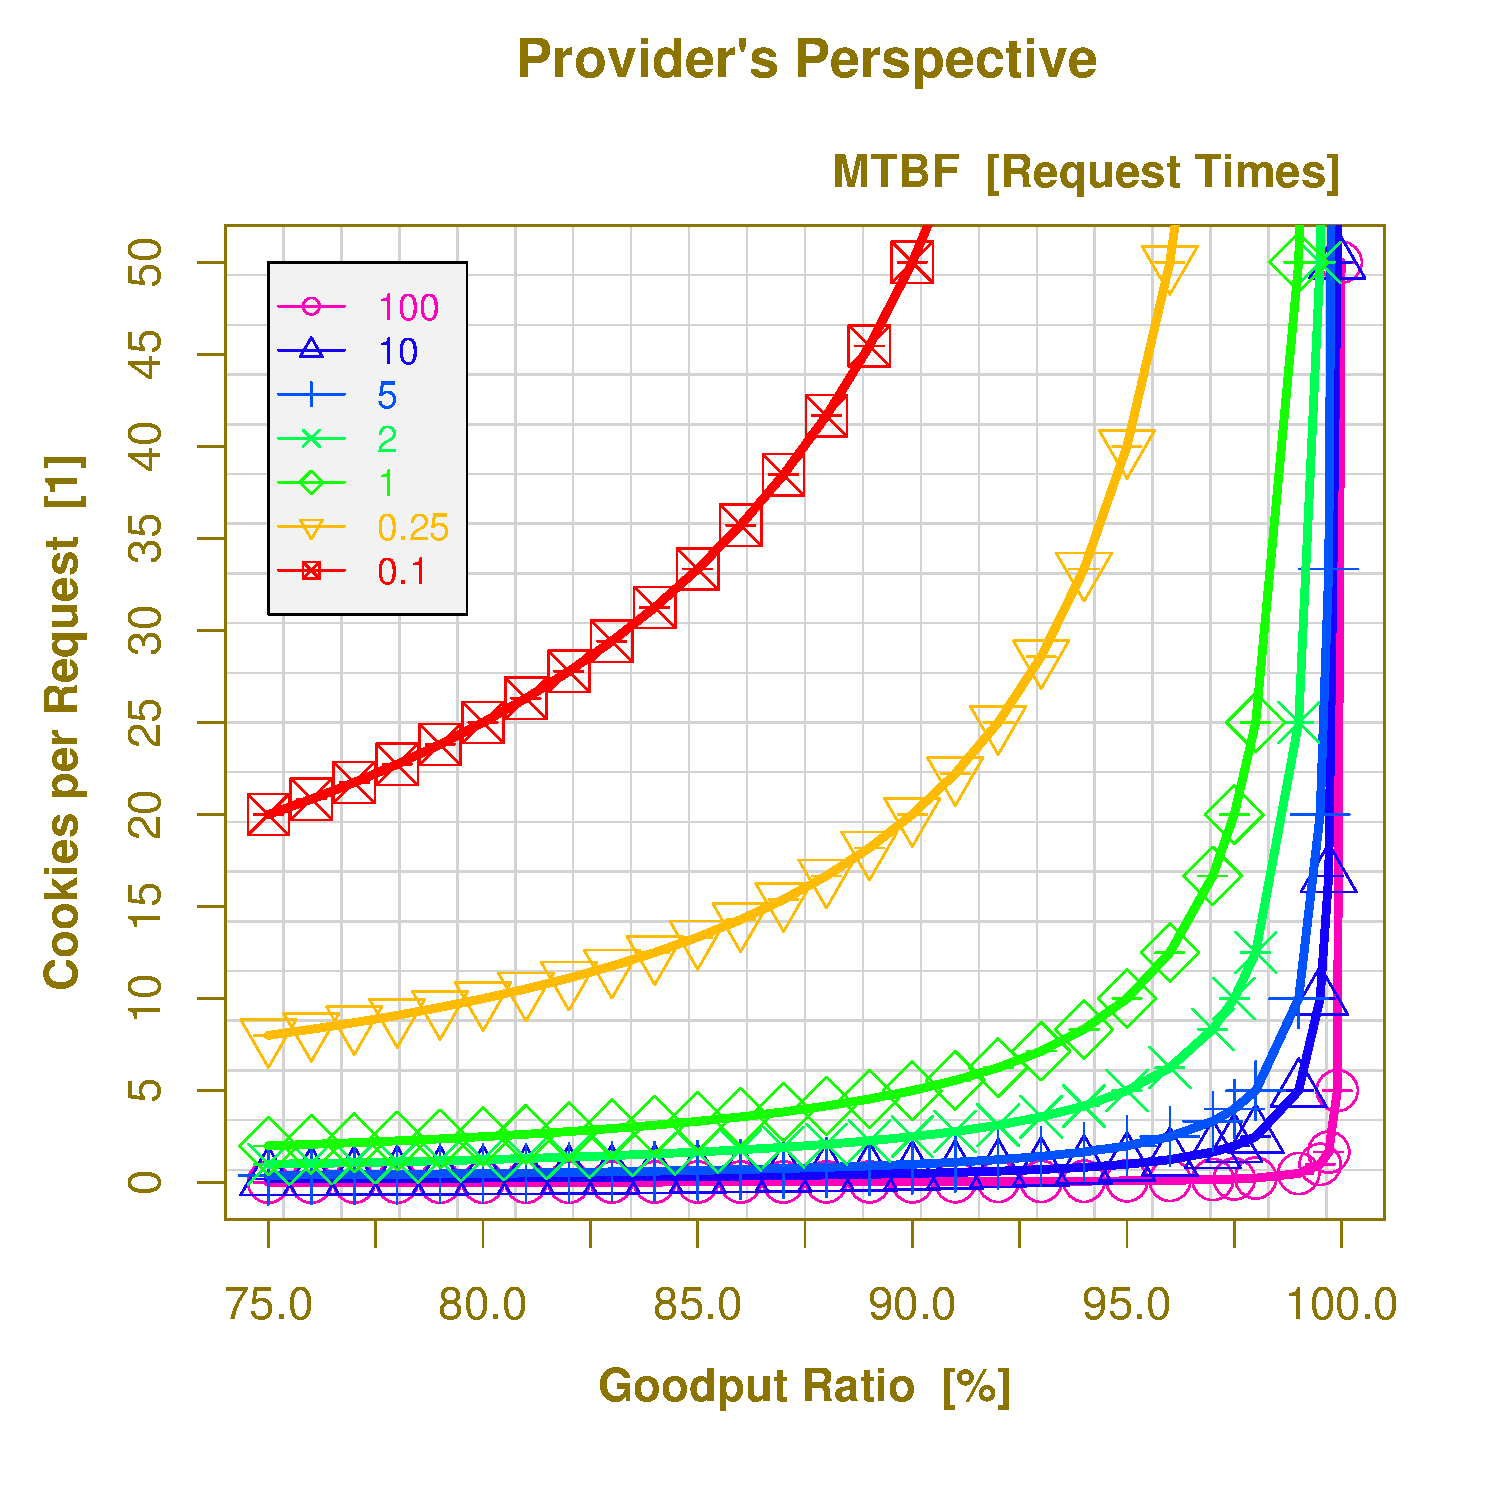
\includegraphics[width=0.60\columnwidth]{%
   Simulations/PDF/test.pdf}
\end{center}
\caption{Simulationsergebnisse}
\label{cap:Simulationsergebnisse}
\end{figure}
% %%%%%%%%%%%%%%%%%%%%%%%%%%%%%%%%%%%%%%%%%%%%%%%%%%%%%%%%%

In Abbildung~\ref{cap:Simulationsergebnisse} sieht man das
Ergebnis der Simulation\index{Simulation}. \emph{Simulation} wird
als Stichwort in den Index geschrieben.

...

...

...



% ###########################################################################
\section{Vierter Abschnitt}
\label{sec:Abschnitt4}
% ###########################################################################

% %%%%%%%%%%%%%%%%%%%%%%%%%%%%%%%%%%%%%%%%%%%%%%%%%%%%%%%%%
\begin{algorithm}
\lstinputlisting{CodeSnippets/Internet16.c}
\caption{The 16-Bit Internet Checksum Algorithm}
\label{alg:The-16-Bit-Internet-Checksum-Algorithm}
\end{algorithm}
% %%%%%%%%%%%%%%%%%%%%%%%%%%%%%%%%%%%%%%%%%%%%%%%%%%%%%%%%%

Algorithmus~\ref{alg:The-16-Bit-Internet-Checksum-Algorithm} zeigt die
Berechnung der 16-Bit-Internet-Checksumme aus~\cite{RFC1071,RFC1624}.


...

...

...



% ###########################################################################
\section{Fünfter Abschnitt}
\label{sec:Abschnitt5}
% ###########################################################################

% %%%%%%%%%%%%%%%%%%%%%%%%%%%%%%%%%%%%%%%%%%%%%%%%%%%%%%%%%
\begin{table}
\begin{center}
\begin{tabular}{|l|l|}
\hline
Problem&
Detection Mechanism
\tabularnewline
\hline
\hline
Congestion&
Sequence Numbers and Acknowledgements
\tabularnewline
\hline
Transmission Error&
Checksum, Packet Drop Extension
\tabularnewline
\hline
Link and Router Problems&
Path Monitoring, Multi-Homing
\tabularnewline
\hline
\end{tabular}
\caption{The Network and Component Failure Detection Mechanisms of SCTP}
\label{tbl:The-Component-Failure-Detection-Mechanisms-of-SCTP}
\end{center}
\end{table}
% %%%%%%%%%%%%%%%%%%%%%%%%%%%%%%%%%%%%%%%%%%%%%%%%%%%%%%%%%

Tabelle~\ref{tbl:The-Component-Failure-Detection-Mechanisms-of-SCTP} zeigt
die Failure-Detection-Mechanismen von SCTP~\cite{RFC2960}.

...

...

...



% ###########################################################################
\section{Sechster Abschnitt}
\label{sec:Abschnitt6}
% ###########################################################################

...

% %%%%%%%%%%%%%%%%%%%%%%%%%%%%%%%%%%%%%%%%%%%%%%%%%%%%%%%%%
\begin{figure}
\begin{center}
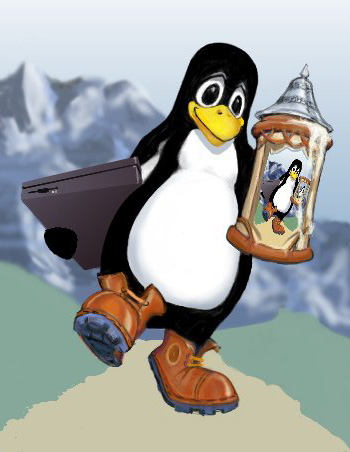
\includegraphics[width=0.40\columnwidth]{%
   Images/PDF/Tux.pdf}
\end{center}
\caption{Rasterbild}
\label{cap:Rasterbild}
\end{figure}
% %%%%%%%%%%%%%%%%%%%%%%%%%%%%%%%%%%%%%%%%%%%%%%%%%%%%%%%%%

In Abbildung~\ref{cap:Rasterbild} sieht man ein Rasterbild\index{Rasterbild} (JPEG-Datei).

...



% ###########################################################################
\section{Summary}
% ###########################################################################

Eine Zusammenfassung.

...
